\let\negmedspace\undefined
\let\negthickspace\undefined
\documentclass[journal]{IEEEtran}
\usepackage[a5paper, margin=10mm, onecolumn]{geometry}
%\usepackage{lmodern} % Ensure lmodern is loaded for pdflatex
\usepackage{tfrupee} % Include tfrupee package

\setlength{\headheight}{1cm} % Set the height of the header box
\setlength{\headsep}{0mm}  % Set the distance between the header box and the top of the text

\usepackage{gvv}
\usepackage{cite}
\usepackage{amsmath,amssymb,amsfonts,amsthm}
\usepackage{algorithmic}
\usepackage{graphicx}
\usepackage{textcomp}
\usepackage{xcolor}
\usepackage{txfonts}
\usepackage{listings}
\usepackage{enumitem}
\usepackage{mathtools}
\usepackage{gensymb}
\usepackage{comment}
\usepackage[breaklinks=true]{hyperref}
\usepackage{tkz-euclide} 
\usepackage{listings}
% \usepackage{gvv}                                        
\def\inputGnumericTable{}                                 
\usepackage[latin1]{inputenc}                                
\usepackage{color}                                            
\usepackage{array}                                            
\usepackage{longtable}                                       
\usepackage{calc}                                             
\usepackage{multirow}                                         
\usepackage{hhline}                                           
\usepackage{ifthen}                                           
\usepackage{lscape}
\newcommand{\begin{eqnarray}
\newcommand{\EEQA}{\end{eqnarray}
\newcommand{\define}{\stackrel{\triangle}{=}}

\begin{document}

\bibliographystyle{IEEEtran}
\vspace{3cm}

\title{1.4.13}
\author{EE24BTECH11021 - Eshan Ray}

% \maketitle
% \newpage
% \bigskip
{\let\newpage\relax\maketitle}

\renewcommand{\thefigure}{\theenumi}
\renewcommand{\thetable}{\theenumi}
\setlength{\intextsep}{10pt} % Space between text and floats



\textbf{Question: }\\
If $\vec a$ and $\vec b$ are the position vectors of $\vec A$ and $\vec B$, respectively, find the position vector
of a point $\vec C$ in $BA$ produced such that $BC = 1\cdot5BA.$\\
\solution{
Point $\vec C$ divides  $BA$ in the ratio $3\colon1$ externally,\\ $\therefore$ using section formula,\\
\begin{align}
	 C&=\frac{kA - B}{k-1} \quad{\brak{where, k=\frac{3}{1}}}\\
	\implies C&=\frac{3A - B}{3 - 1}\\
	\implies C&=\frac{3a - b}{2}\\
	\implies C&=1\cdot5a-0\cdot5b
 \end{align}
So, position vector of $\vec C$ is $1\cdot5\vec a-0\cdot5\vec b$.}
\begin{figure}[!ht]
    \centering
	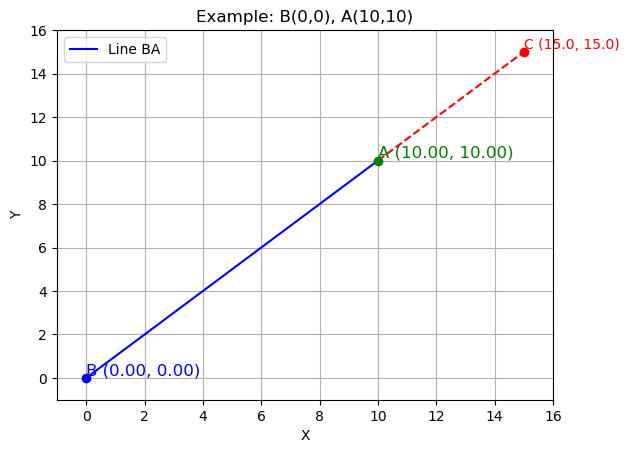
\includegraphics[width=1\textwidth]{plots/plot.png}
    \caption{ Coordinates of C}
    \label{fig:plot}
\end{figure}
\end{document}





 





